\documentclass[11pt, oneside]{article} 
\usepackage{geometry}
\geometry{letterpaper} 
\usepackage{graphicx}
	
\usepackage{amssymb}
\usepackage{amsmath}
\usepackage{parskip}
\usepackage{color}
\usepackage{hyperref}

\graphicspath{{/Users/telliott/Dropbox/Github-Math/quickgeo/figures/}{/Users/telliott/Dropbox/Github-Math/figures/}}
% \begin{center} \includegraphics [scale=0.4] {gauss3.png} \end{center}

\title{Area}
\date{}

\begin{document}
\maketitle
\Large

%[my-super-duper-separator]

Area is defined by squares of whatever unit size we choose, whether it's square miles (miles${^2}$) or nanometers (nm${^2}$) or something in between, like inches (in${^2}$), or centimeters (cm${^2}$).

In the simplest cases, the area to be computed is that of a rectangle or a square, and the lengths of the sides are an even multiple of our unit length.  

 \begin{center} 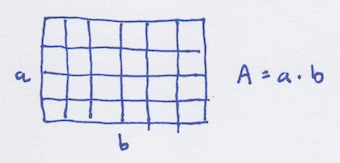
\includegraphics [scale=0.5] {E1.png} \end{center}
In the example above $a = 4$ and $b = 6$ and the area is
\[ A = a \cdot b = 4 \cdot 6 = 24 \]

We are interested in finding the areas of different triangles.

In a famous essay, Lockhart says that it is a mistake (an error in teaching) to just give the formula to begin with.  

\url{https://www.maa.org/sites/default/files/pdf/devlin/LockhartsLament.pdf}

Instead, what we should do to appreciate the art of geometry is to draw a triangle in a box, like this
\begin{center} 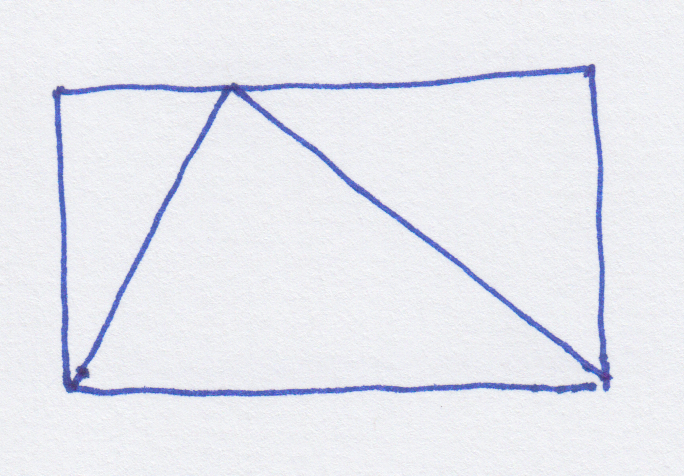
\includegraphics [scale=0.7] {E10.png} \end{center}
and then wonder, or guess, what the area is inside the triangle compared to the surrounding box.  

The "aha" moment comes when we draw a vertical down, and see that the two smaller triangles are exactly one-half of their surrounding boxes.
\begin{center} 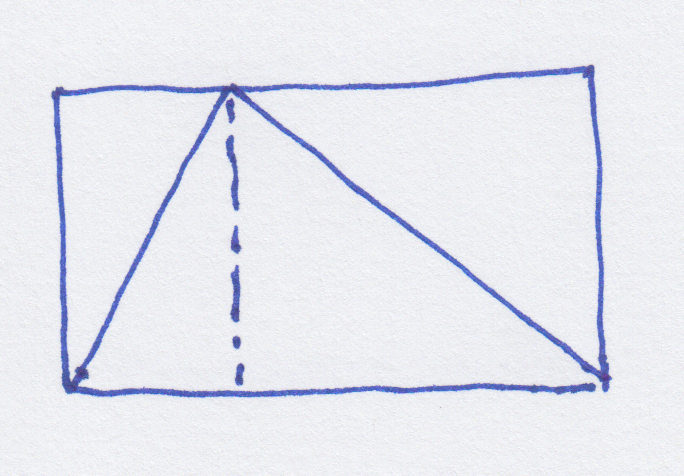
\includegraphics [scale=0.7] {E11.png} \end{center}
Aha!  

This is characteristic of many proofs, as you may notice.  A line is extended or a new line drawn at a point and parallel to some other line.  The drawing we start with gets enhanced, and then you suddenly see the way forward.

So how do we know that the diagonal cuts a rectangle into two equal parts?  One answer:  symmetry.  There is no reason to favor one piece over the other.  Or use the properties of rectangles in the following way.

\subsection*{systematic approach}

Any rectangle can be divided by drawing its diagonal.  The result is two right triangles, and these two triangles are congruent.

In the drawing, all four vertices are right angles (this is a rectangle), but only one is marked as such.
\begin{center} 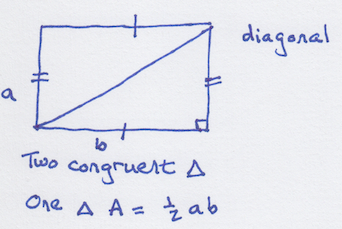
\includegraphics [scale=0.6] {E2.png} \end{center}
Since the area of the whole is $a \cdot b$ and we have produced two identical halves, the area of each right triangle is 
\[ A_{\triangle} = \frac{ab}{2} \]

This is true for \emph{any} right triangle.  
\begin{center} 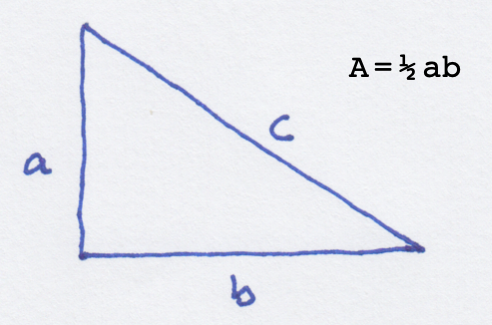
\includegraphics [scale=0.3] {E12.png} \end{center}
The longest side in a right triangle is called the hypotenuse.  The product of the other two sides, times one-half, is the area of any right triangle.

It is mildly annoying to keep track of that factor of one-half all the time.  A solution, which we will follow for the rest of this chapter, is to talk about \emph{twice} the area of the triangle, and say that
\[ 2A_{\triangle} = ab \]

Now, suppose we do not have a right triangle, but a line drawn from the top vertex down to the base (called the \emph{altitude}), perpendicular to it, and that line stays inside the triangle.   
\begin{center} 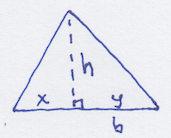
\includegraphics [scale=0.8] {E4.png} \end{center}

Then the altitude $h$ divides the triangle into two smaller right triangles.  The total area is the sum of those smaller triangles.
\[ 2A = hx + hy =  h(x + y) =  hb \]

In the diagram below, if we would move the top vertex back and forth along a line parallel to the base, the height would not change, and neither would the area of the triangle.
\begin{center} 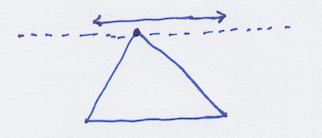
\includegraphics [scale=0.6] {E5.png} \end{center}

$\bullet$ \ Triangles with the same base length and a vertex anywhere on a line parallel to the base, have equal areas.

This approach still works for an obtuse triangle.  In that case, if the largest angle is one of the base angles, then a line dropped perpendicular to the base, meets the base outside of the triangle.  An easy way to see that the formula still works is to compute the areas of the two right triangles in the figure.
\begin{center} 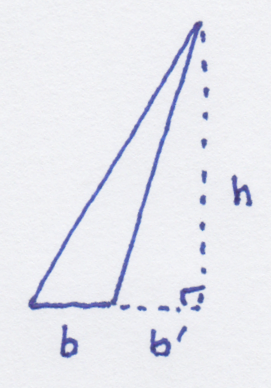
\includegraphics [scale=0.4] {E6.png} \end{center}

The base of the triangle is $b$ and the short dotted line which extends $b$ to meet the vertical line is $b'$.  Twice the area of the large right triangle is $h(b + b')$  and twice the area of the small dotted right triangle is $A = ab'$.  The area of the original triangle is the difference.
\[ A = a(b+b') - ab' = ab \]

\subsection*{a different view}

Another way to think about the area of triangles is to start with a parallelogram, which is a quadrilateral (four-sided figure) with both pairs of opposite sides parallel.  

As a consequence the opposing sides and angles are equal.  Angles that flank one another add up to 180. 
\begin{center} 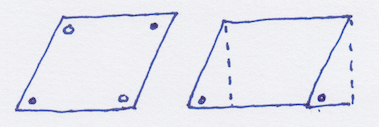
\includegraphics [scale=0.8] {E7a.png} \end{center}

The area of a parallelogram is the base times the length of a perpendicular from one vertex to the base, or an extension of the base.  You can see that this works by cutting off a small triangle on one end and attaching it at the other.

But any triangle can be converted into a parallelogram, by drawing a congruent triangle, turning it around, and pasting them together, as shown.
\begin{center} 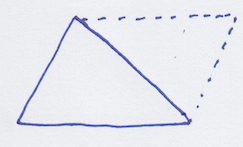
\includegraphics [scale=0.6] {E8.png} \end{center}
So the area is the base times the vertical height, times one-half since there are two copies of the original triangle.

For an obtuse triangle, the parallelogram may lean over so far that you can't easily turn it into a rectangle.

However, this difficulty can be solved by dividing the parallelogram into sections horizontally.  Each individual section can be converted to a rectangle, and the areas added up for the pieces.
\begin{center} 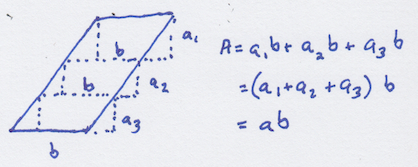
\includegraphics [scale=0.6] {E9.png} \end{center}

\subsection*{note}

The area of a triangle must be the same no matter which side we choose as the base.  

We won't go through the proof in detail, but by cutting the triangle up into smaller ones, we can show that $af = ch$ (and $b$ times its altitude is also equal, as well).

\begin{center} 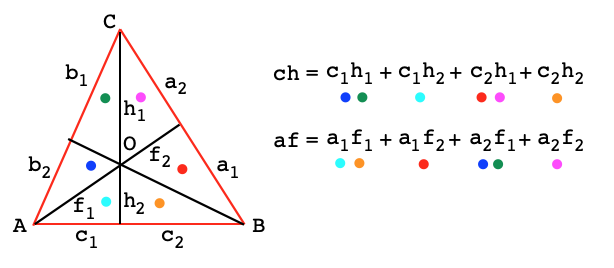
\includegraphics [scale=0.5] {area8b.png} \end{center}

\subsection*{area-ratio theorem}

A triangle is divided into two smaller ones by drawing a line from the top vertex to some arbitrary point along the base.  Since both triangles have the same altitude (a perpendicular from the apex), twice the areas are in the same ratio as the bases.
\begin{center} 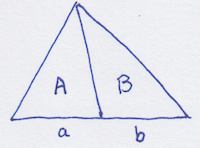
\includegraphics [scale=0.8] {E13.png} \end{center}
\[ \frac{(2A)}{(2B)} = \frac{ha}{hb} = \frac{a}{b} \]

Now we take an arbitrary triangle and draw the angle bisector at the top, splitting the base into $a$ and $b$.  The right triangles that are formed by the dotted line are congruent.  We have two angles (thus three angles) and the shared side. 
\begin{center} 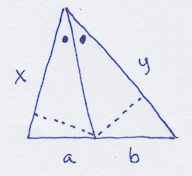
\includegraphics [scale=0.8] {E14.png} \end{center}
So let the dotted line be $h$ and then
\[ \frac{(2A)}{(2B)} = \frac{(A)}{(B)} = \frac{hx}{hy} = \frac{x}{y} \]

But the area-ratio theorem also applies, giving
\[ \frac{(2A)}{(2B)} = \frac{(A)}{(B)} = \frac{a}{b} = \frac{x}{y} \]
which also means
\[ \frac{x}{a} = \frac{y}{b} \]

\end{document}
